\documentclass[11pt,a4paper]{article}
\usepackage[T1]{fontenc}
\usepackage[utf8]{inputenc}
\usepackage{lmodern,microtype,amsmath,amssymb,booktabs,longtable,array,graphicx}
\usepackage[margin=23mm]{geometry}
\usepackage{xcolor,tikz,fancyhdr,enumitem}
\usetikzlibrary{arrows.meta,positioning}
\definecolor{navy}{HTML}{0F1E2E}
\definecolor{teal}{HTML}{0D8080}
\definecolor{ice}{HTML}{EEF5F5}
\usepackage[colorlinks=true,linkcolor=teal,urlcolor=teal,citecolor=teal]{hyperref}
\hypersetup{pdftitle={Mini-IPHOREOS Extended System: Mathematical Model of the Cognitive Extension},pdfauthor={Mini-IPHOREOS project}}
\pagestyle{fancy}\fancyhf{}\fancyhead[L]{\small\textcolor{teal}{MINI-IPHOREOS EXTENDED SYSTEM / MATHEMATICAL COMPANION}}
\fancyfoot[L]{\small From joint belief to a receding-horizon decision}\fancyfoot[R]{\thepage}
\setlength{\headheight}{15pt}
\setlength{\parindent}{0pt}\setlength{\parskip}{6pt}
\setlist{itemsep=3pt,topsep=4pt}
\newcommand{\code}[1]{\texttt{\detokenize{#1}}}
\setlength{\emergencystretch}{2em}
\newcommand{\tutoext}[2]{\par\textcolor{teal}{\textbf{Do this in the Extended-system tutorial:}} Section #1, #2. See \href{Tutorial_EXT1_EN.html}{the browser tutorial} or \href{Tutorial_EXT1_EN.pdf}{the PDF tutorial}.\par}
\newcommand{\tutoVone}[2]{\par\textcolor{teal}{\textbf{Shared with the Baseline system:}} see \href{baseline_v1/Mathematical_Model.pdf}{\code{baseline_v1/Mathematical_Model.pdf}}, #1, #2.\par}
\newcommand{\N}{\mathcal N}
\begin{document}
\begin{titlepage}
\textcolor{teal}{\large IPHOREOS / CONCEPT--EVENT--CONTEXT--POLICY}\par
\vspace{14mm}
{\Huge\bfseries\color{navy} The mathematical model\\[3mm] of the Extended system\par}
\vspace{5mm}
{\Large Joint distance/speed belief, inferred context, information-seeking and a receding-horizon decision\par}
\vspace{7mm}
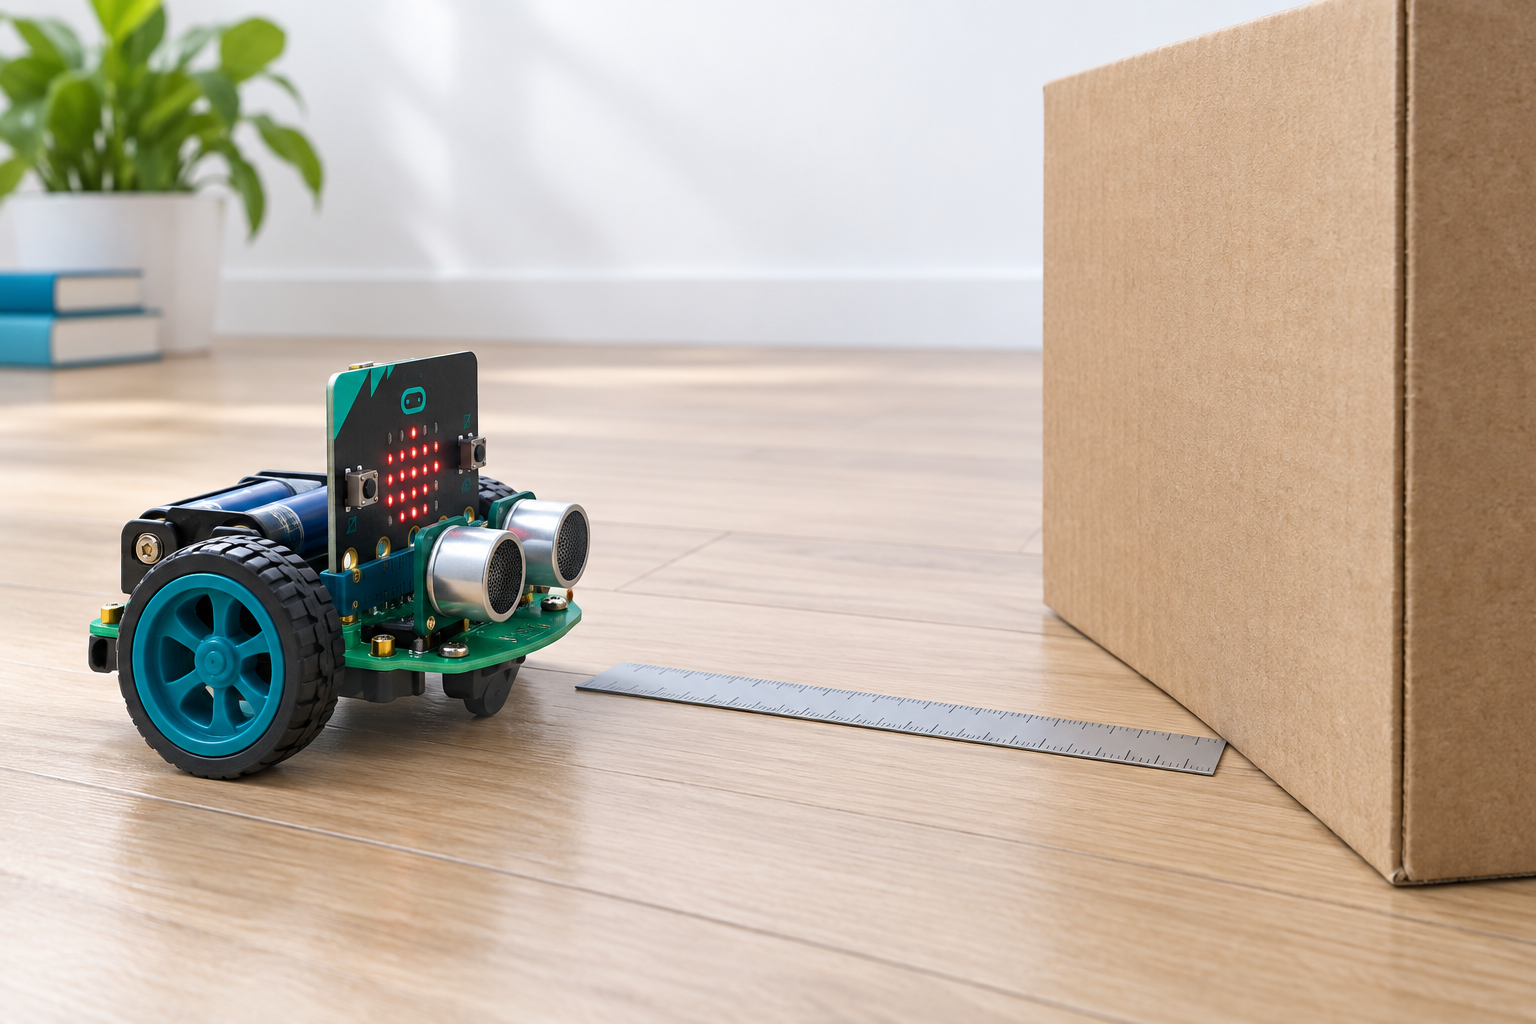
\includegraphics[width=\linewidth,height=70mm,keepaspectratio]{baseline_v1/assets/robot_concept.png}
\par{\small AI-generated concept illustration, shared with the Baseline system; not a photograph or an assembly drawing.\par}
\vspace{7mm}
\colorbox{ice}{\parbox{.95\linewidth}{\textbf{Same observable task as the Baseline system.} Approach a cardboard wall and verify that the ultrasonic sensor face is within 21--29 cm of it, with a nominal target of 25 cm. The Extended system changes how the controller estimates state and decides, not the task or the hardware interface.}}\par
\vspace{5mm}
This companion derives the equations behind every change the Extended system (\code{EXT1}) makes over the Baseline system (\code{V1}), across four
milestones: a two-mode joint distance/speed belief, a Gaussian information proxy, a
two-step receding-horizon planner with an explicit no-progress cost, and a fair
rule-based comparator (Milestone~1); a persistent per-context memory, the diagnosed
reason it alone did not help, and the accumulated-evidence recognition mechanism that
then made it work (Milestone~2, Sections~\ref{sec:memory-negative}--\ref{sec:cusum});
an explicit, costed sensor-bias reference that breaks the distance/bias
identifiability problem (Milestone~3, Section~\ref{sec:bias-ref}); and a frozen
evaluation on genuinely held-out seeds, plus a new outlier-reading robustness test
(Milestone~4, Section~\ref{sec:heldout}); and a later, separate validation pass, the
\emph{Transfer system}, testing whether the learned context library transfers to a
different goal under a persistent, deployment-specific speed bias
(Section~\ref{sec:transfer}) -- positive preliminary evidence for faster regime
recognition across tasks, reported together with the metrics it does not move, not
folded into the four-milestone count above. It assumes familiarity with \code{baseline_v1/Mathematical_Model.pdf} for the shared sensor model and the physical pulse-to-motor mapping, which are not re-derived here.

\textbf{Start with:} \href{Tutorial_EXT1_EN.pdf}{the Extended-system tutorial} or \href{README.md}{the Extended-system README}. Keep this PDF beside those files so relative links resolve.

\vfill
Prepared for Florent Ouabo Kamkumo\\
3 October 2026 / Extended System Milestone 4 companion v4.0\\
\textbf{Status:} computer-tested desktop prototype; no physical validation. All six
items of the project's improvement plan are now addressed (Section~\ref{sec:next});
physical hardware validation remains entirely separate and not yet attempted.
\end{titlepage}
\tableofcontents
\newpage

\section{The task and what the Extended system adds}
The Baseline system answers: \emph{given an uncertain distance measurement and an imperfect movement model, should the robot move a little, measure again, or stop?} with a scalar Bayesian estimator and a one-step rule. The Extended system answers a richer question: \emph{given uncertain distance \textbf{and} speed, under one of several possible movement contexts, what short sequence of actions over the next few decisions best balances progress, cost and the value of more information?}

Three extensions are layered on the shared observation model and verification rule (Sections~\ref{sec:shared}--\ref{sec:verify} summarise what is shared; Sections~\ref{sec:horizon}--\ref{sec:fair} derive what is new):
\begin{enumerate}
\item A joint state $(d,v)$ -- distance and effective speed -- tracked as a weighted mixture of Gaussians, one per movement context (normal/slow), rather than a single scalar.
\item A Gaussian information proxy that can reward an action for the speed uncertainty it is expected to resolve, not only for reducing distance error.
\item \textbf{New this release.} A receding-horizon planner that scores short (two-decision) action sequences instead of one decision at a time, with an explicit penalty for sequences that make no progress, and a fair rule-based comparator (\code{FairRuleBaseline}) that gives the Baseline system's decision philosophy the same action menu as the Extended system, so that any remaining performance gap is attributable to the decision architecture rather than to a richer set of available actions.
\end{enumerate}

\textbf{The one-cycle shape of everything below.} Before the equations, the loop every
section after this one is a piece of:
\begin{center}
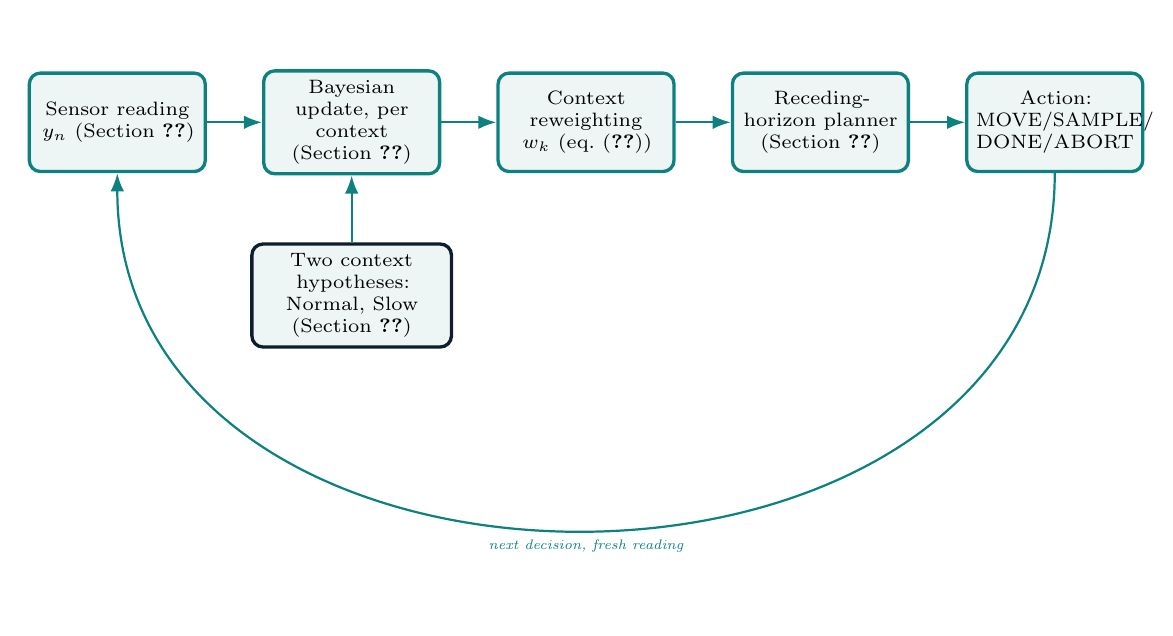
\begin{tikzpicture}[
  box/.style={rectangle,rounded corners,draw=teal,very thick,fill=ice,text width=2.0cm,align=center,minimum height=1.25cm,font=\scriptsize},
  hyp/.style={rectangle,rounded corners,draw=navy,very thick,fill=ice,text width=2.3cm,align=center,minimum height=1.05cm,font=\scriptsize},
  arr/.style={-{Latex[length=2.3mm]},thick,teal}
]
\node[box] (sensor) {Sensor reading $y_n$ (Section~\ref{sec:obs})};
\node[box,right=0.7cm of sensor] (update) {Bayesian update, per context (Section~\ref{sec:update})};
\node[box,right=0.7cm of update] (reweight) {Context reweighting $w_k$ (eq.~\eqref{eq:reweight})};
\node[box,right=0.7cm of reweight] (plan) {Receding-horizon planner (Section~\ref{sec:horizon})};
\node[box,right=0.7cm of plan] (action) {Action: MOVE/SAMPLE/\\DONE/ABORT};
\node[hyp,below=0.85cm of update] (hyp) {Two context hypotheses: Normal, Slow (Section~\ref{sec:movement})};
\draw[arr] (sensor) -- (update);
\draw[arr] (update) -- (reweight);
\draw[arr] (reweight) -- (plan);
\draw[arr] (plan) -- (action);
\draw[arr] (hyp) -- (update);
\draw[arr] (action.south) to[out=-90,in=-90,looseness=1.3] node[below,font=\tiny\itshape]{next decision, fresh reading} (sensor.south);
\end{tikzpicture}
\end{center}
\textit{\small One decision = one pass around this loop. Every section below derives one box or
one arrow; the box/arrow it derives is named in each section's own heading.}
\tutoext{1}{The Extended system: what changes}

\section{Variables and the augmented belief}
\label{sec:shared}
Work in centimetres and seconds, as in the Baseline system. The augmented state per context $k\in\{1,\dots,K\}$ ($K=2$ for \{normal, slow\}, or $K=1$ for the context-free \code{adaptive} variants) is
\[
x_k=(d_k,v_k)^\top,\qquad P_k\in\mathbb R^{2\times2}_{\succeq0},\qquad w_k\in[0,1],\ \textstyle\sum_k w_k=1.
\]
\colorbox{ice}{\parbox{.95\linewidth}{\small\textbf{Example, in plain numbers, before the symbol table below.} The robot starts
roughly 70~cm from the wall and takes its first reading: 69.4~cm (noisy, true sensor
sd $\approx1.2$~cm). With no speed evidence yet, the belief holds \emph{two} running
guesses side by side, weighted by the fixed starting split (0.8/0.2, Section~\ref{sec:movement}):
a "normal" guess $x_{\rm normal}=(69.4,\,8.0)$ -- 69.4~cm, 8.0~cm/s, the calibrated
default speed -- with weight $w_{\rm normal}=0.8$; and a "slow" guess
$x_{\rm slow}=(69.4,\,3.0)$ with weight $w_{\rm slow}=0.2$. After a move and a second
reading, whichever guess's predicted distance matches what was actually observed
starts winning weight (Section~\ref{sec:update}'s reweighting rule) -- within a
handful of readings one $w_k$ is close to 1 and the other close to 0. Every
$d_k,v_k,w_k$ in the rest of this companion is exactly this: not an abstract symbol,
but one of these two running, per-context guesses, updated one reading at a time.}}\par\vspace{4pt}
\begin{longtable}{p{.15\linewidth}p{.57\linewidth}p{.18\linewidth}}
\toprule Symbol & Meaning & Unit\\\midrule\endhead
$d_k,v_k$ & Per-context mean distance and effective speed & cm, cm/s\\
$P_k$ & Per-context $2\times2$ covariance of $(d_k,v_k)$ & cm$^2$, cm$^2$/s, cm$^2$/s$^2$\\
$w_k$ & Posterior probability of context $k$ & dimensionless\\
$\bar x,\bar P$ & Mixture (reported) mean and covariance, eq.~\eqref{eq:moments} & as above\\
$\rho$ & Speed mean-reversion rate per move (0.80 with contexts, 1 without) & dimensionless\\
$Q_d,Q_v$ & Added distance/speed process variance per move & cm$^2$, cm$^2$/s$^2$\\
$T$ & Context transition matrix, fixed at $\mathrm{diag}(.96)+.04(1-\mathrm{diag})$ & dimensionless\\
$H$ & Planning horizon (2 decisions in this release) & dimensionless\\
$\Delta_{\min}$ & No-progress displacement threshold (1 cm) & cm\\
$\lambda$ & No-progress penalty magnitude (1.0, same units as the score) & dimensionless\\
\bottomrule
\end{longtable}
This augments, rather than replaces, the Baseline system's scalar $(\mu,P)$: setting $K=1$ and dropping $v$ recovers a model of the same shape as the Baseline system's belief.
\tutoVone{Section 2}{Variables, units and the complete internal state}

\section{Observation model}
\label{sec:obs}
The Extended system keeps the Baseline system's bias-corrected linear-Gaussian observation model for distance,
\[
y_n=d_n+(b-\hat b)+\nu_n,\qquad \nu_n\overset{\rm model}\sim\N(0,R),
\]
applied identically to every context's distance component; speed is never observed directly, only inferred through its effect on successive distance predictions. The innovation gate rejects an observation when $|y_n-\bar d^-|>5\sqrt{\bar P^-_{dd}+R}$ (five standardised units; a widened version of the Baseline system's $\max\{8,4\sqrt{P^-+R}\}$ cm rule, since the reference implementation (\code{cognitive/model.py}, \code{Belief.observe}) expresses the test directly in standardised, not raw, units). \code{FairRuleBaseline} (Section~\ref{sec:fair}) instead reuses the Baseline system's exact raw-unit test, since it is a rule-based comparator, not an estimator of speed.
\tutoVone{Section 3}{From ultrasound time to a distance observation}

\section{Context-mixture movement model}
\label{sec:movement}
Conditional on context $k$ being active and a pulse of duration $\tau$,
\begin{equation}\label{eq:gen}
d_{k,n+1}=d_{k,n}-v_{k,n}\tau-c+w^d_n,\qquad
v_{k,n+1}=\rho\,v_{k,n}+(1-\rho)m_k+w^v_n,
\end{equation}
where $c$ is coast distance and $m_k$ is context $k$'s calibrated nominal speed (about 8 and 3 cm/s for normal and slow). Context itself follows a fixed Markov chain with transition matrix $T$ ($T_{kk}=.96$, off-diagonal $.04$ for $K=2$), applied once per \emph{motor} decision, not once per stationary reading -- repeated SAMPLE actions leave $w_k$ unchanged by this mechanism (verified by \code{test_stationary_sampling_does_not_identify_speed}).

\textbf{What "a weighted mixture of Gaussians, one per context" looks like.} Section~\ref{sec:shared}'s opening phrase, drawn rather than only stated -- two candidate speed beliefs held at once, each a bump of uncertainty around its own current mean, scaled here by the starting weights $w_{\rm normal}=0.8,w_{\rm slow}=0.2$ (sketch only, not to the filter's actual calibrated scale):
\begin{center}
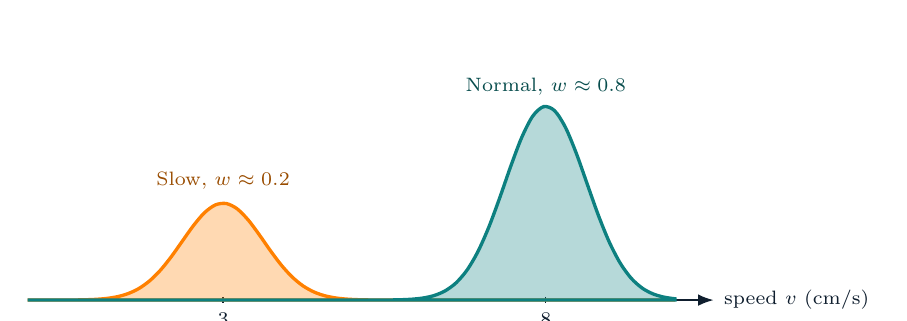
\begin{tikzpicture}[scale=0.82]
\draw[-{Latex[length=2mm]},thick,navy] (0,0) -- (10.6,0) node[right,font=\scriptsize]{speed $v$ (cm/s)};
\draw[navy] (3,0.05) -- (3,-0.05) node[below,font=\scriptsize]{3};
\draw[navy] (8,0.05) -- (8,-0.05) node[below,font=\scriptsize]{8};
\draw[orange,very thick,fill=orange,fill opacity=0.3,domain=0:10,samples=60,smooth]
  plot ({\x},{1.5*exp(-((\x-3)*(\x-3))/0.8)}) -- (10,0) -- (0,0) -- cycle;
\draw[teal,very thick,fill=teal,fill opacity=0.3,domain=0:10,samples=60,smooth]
  plot ({\x},{3.0*exp(-((\x-8)*(\x-8))/0.8)}) -- (10,0) -- (0,0) -- cycle;
\node[orange!60!black,font=\scriptsize] at (3,1.85) {Slow, $w\approx0.2$};
\node[teal!60!black,font=\scriptsize] at (8,3.3) {Normal, $w\approx0.8$};
\end{tikzpicture}
\end{center}
As readings arrive, eq.~\eqref{eq:reweight} shifts weight toward whichever bump better predicts them (narrowing toward one spike, Section~\ref{sec:update}); eq.~\eqref{eq:imm-mix}--\eqref{eq:advance} below is what moves and reshapes each bump between readings.

\textbf{Moment-matching mixture collapse.} Before propagating, the implementation (\code{Belief._advance}) first mixes each outgoing context $j$'s prior moments over all incoming contexts $i$, weighted by $w_i T_{ij}/w_j^-$ where $w^-=wT$ is the predicted context prior:
\begin{equation}\label{eq:imm-mix}
\tilde w_{i\to j}=\frac{w_i T_{ij}}{w_j^-},\qquad
\tilde x_j=\sum_i \tilde w_{i\to j}\,x_i,\qquad
\tilde P_j=\sum_i \tilde w_{i\to j}\Bigl(P_i+(x_i-\tilde x_j)(x_i-\tilde x_j)^\top\Bigr).
\end{equation}
This is the interacting-multiple-model (IMM) mixing step: it lets a context's belief absorb information from other contexts in proportion to how likely a transition from each of them was, rather than keeping $K$ fully independent filters. Equation~\eqref{eq:gen} is then applied per context to $(\tilde x_j,\tilde P_j)$, giving the linear update
\begin{equation}\label{eq:advance}
x_j'=F_\tau\,\tilde x_j+\begin{pmatrix}-c\\(1-\rho)m_j\end{pmatrix},\qquad
P_j'=F_\tau\,\tilde P_j\,F_\tau^\top+\mathrm{diag}(Q_d,Q_v),\qquad
F_\tau=\begin{pmatrix}1&-\tau\\0&\rho\end{pmatrix}.
\end{equation}
\code{Belief.predict} applies \eqref{eq:imm-mix}--\eqref{eq:advance} in place; \code{Belief.predicted} (new this release) returns the same result \emph{without} mutating the stored belief, and \code{Belief._advance} is the pure function both call -- this is what lets the planner (Section~\ref{sec:horizon}) roll the belief forward hypothetically, more than one step, without disturbing the real filter. The reported (mixture) mean and covariance at any point are
\begin{equation}\label{eq:moments}
\bar x=\sum_k w_k x_k,\qquad
\bar P=\sum_k w_k\bigl(P_k+(x_k-\bar x)(x_k-\bar x)^\top\bigr).
\end{equation}
\tutoext{3}{Model and estimation}

\section{Bayesian update and context reweighting}
\label{sec:update}
On an accepted reading $y_n$, each context's distance component is updated by an ordinary Kalman step with gain $g_k=P_k[:,0]/(P_{k,dd}+R)$, applied to the full 2-vector $x_k$ (so a distance innovation also nudges the speed estimate through the off-diagonal of $P_k$, which is exactly how a single move followed by a reading lets the filter learn about speed from distance alone). The implementation applies the update in Joseph form for numerical robustness,
\[
x_k\leftarrow x_k+g_k(y_n-d_k),\qquad
P_k\leftarrow(I-g_ke_1^\top)P_k(I-g_ke_1^\top)^\top+g_kg_k^\top R,\qquad e_1=(1,0)^\top.
\]
Context weights update by their per-context marginal likelihood, exactly as a Gaussian-mixture filter's weights:
\begin{equation}\label{eq:reweight}
\ell_k=\log w_k-\tfrac12\Bigl[\log(2\pi(P_{k,dd}+R))+\frac{(y_n-d_k)^2}{P_{k,dd}+R}\Bigr],\qquad
w_k\leftarrow\frac{e^{\ell_k-\max_j\ell_j}}{\sum_je^{\ell_j-\max_j\ell_j}}.
\end{equation}
The $\max_j\ell_j$ subtraction is a standard log-sum-exp stabiliser; it does not change the normalised result. A context that predicts the observed reading much better than the other accumulates weight geometrically fast; this is the mechanism behind \code{test_context_inference_and_covariance}, which checks that forty-five slow-context observations drive $w_{\rm slow}>0.8$.
\tutoVone{Section 5}{Deriving the scalar Bayesian update}

\section{The information proxy}
\label{sec:info}
For a hypothetical pulse of duration $\tau$ (evaluated on the \emph{current}, not mixture-mixed, state, via \code{Belief.information}), approximate the one-step-ahead joint covariance as $P^+=F_\tau\bar PF_\tau^\top+\mathrm{diag}(Q_d,Q_v)\mathbf 1_{\tau>0}$. The value of a subsequent distance reading for \emph{speed} is captured by comparing the marginal speed variance before and after conditioning on a hypothetical distance observation:
\[
P^+_{\rm post}=\max\Bigl(10^{-9},\,P^+_{vv}-\frac{(P^+_{vd})^2}{P^+_{dd}+R}\Bigr),\qquad
\mathrm{Info}(\tau)=\max\Bigl(0,\,\tfrac12\log\frac{P^+_{vv}}{P^+_{\rm post}}\Bigr).
\]
This is the differential entropy reduction of a Gaussian under a linear-Gaussian observation, restricted to the speed marginal; it is a proxy for the value of information about speed specifically, not an expected free energy functional and not a measure of information about context (which would require comparing full mixture predictive distributions across hypotheses, not a single Gaussian's conditional variance). $\mathrm{Info}(0)=0$ since $F_0=I$ and no process noise is added, so SAMPLE never buys speed information in this proxy -- consistent with speed only ever being learned through move-then-observe pairs (Section~\ref{sec:movement}).
\tutoext{3}{Model and estimation}

\section{The one-step planner this release replaces}
\label{sec:old}
Through the previous Extended-system release, each decision scored the three candidate durations $\tau\in\{0,.12,.24\}$ once, using a closed-form one-step approximation
\[
\widehat P(\tau)=\bar P_{dd}-2\tau\bar P_{dv}+\tau^2\bar P_{vv}+Q_d\mathbf 1_{\tau>0},\qquad
\mathrm{Score}_1(\tau)=\frac{(\bar d-v\tau-25)^2+\widehat P(\tau)}{400}+0.08\,\kappa(\tau)-0.8\,\mathrm{Info}(\tau),
\]
with $\kappa(\tau)=\tau+.20$ for a move and $\kappa(0)=.15$ for SAMPLE, and $\tau$ excluded if $\bar d-v\tau-2.33\sqrt{\widehat P(\tau)}-.5<21$. This is a one-step, closed-form approximation to the mixture dynamics (it operates on aggregate moments directly, not through \eqref{eq:imm-mix}--\eqref{eq:advance}). Because it only ever compares \emph{this instant's} alternatives, a state in which every SAMPLE-vs-MOVE trade-off narrowly favours SAMPLE -- for instance because remaining distance uncertainty is already small and a move's added process variance $Q_d$ outweighs its small expected progress -- has no mechanism to recognise that committing to a plan which samples now and moves next is preferable to sampling indefinitely. With information-seeking switched off ($\mathrm{Info}\equiv0$ in the score), this could make the all-SAMPLE action a persistent local optimum. Section~\ref{sec:horizon} replaces $\mathrm{Score}_1$ with a two-step, forward-simulated score that both uses the real mixture dynamics and adds an explicit term for this specific failure mode.

\section{The receding-horizon planner}
\label{sec:horizon}
At each decision, enumerate every pair $(\tau_1,\tau_2)\in\{0,.12,.24\}^2$ ($H=2$, nine pairs). For each pair, roll the belief forward twice using \eqref{eq:imm-mix}--\eqref{eq:advance} without mutating it (\code{Belief.predicted} then \code{Belief._advance}), obtaining mixture moments $(\bar d_1,\bar P_1)$ after the first step and $(\bar d_2,\bar P_2)$ after the second. Exclude a pair the moment either half-step would predict an unsafe overshoot,
\[
\tau_i>0\ \text{and}\ \bar d_i-2.33\sqrt{\bar P_{i,dd}}-.5<21\quad\Longrightarrow\quad\text{exclude }(\tau_1,\tau_2).
\]
Among the surviving pairs, score
\begin{equation}\label{eq:horizon-score}
\mathrm{Score}_2(\tau_1,\tau_2)=\underbrace{\frac{(\bar d_2-25)^2+\bar P_{2,dd}}{400}}_{\text{end-of-horizon goal}}
+\underbrace{0.08\,\kappa(\tau_1)+0.08\,\kappa(\tau_2)}_{\text{accumulated cost}}
-\underbrace{0.8\,\mathrm{Info}(\tau_1)}_{\text{information, first step only}}.
\end{equation}
Information is evaluated only for $\tau_1$ (the action about to be executed), matching the principle that information-seeking should improve an already competent controller rather than substitute for one: the end-of-horizon goal term, not a speculative two-step information term, is what the no-progress correction below targets.

\textbf{Explicit no-progress cost.} Let $\Delta(\tau_1,\tau_2)=\bar d-\bar d_2$ be the pair's net predicted displacement from the current mean $\bar d$. If \emph{some} surviving pair achieves $\Delta>\Delta_{\min}=1$~cm, add a fixed penalty $\lambda=1.0$ to the all-SAMPLE pair's score:
\begin{equation}\label{eq:no-progress}
\mathrm{Score}_2(0,0)\ \leftarrow\ \mathrm{Score}_2(0,0)+\lambda\cdot\mathbf 1\Bigl[\max_{(\tau_1,\tau_2)}\Delta(\tau_1,\tau_2)>\Delta_{\min}\Bigr].
\end{equation}
Execute $\tau_1^\star$ from $\arg\min\mathrm{Score}_2$ (receding-horizon control: only the first action is taken; the next decision re-plans from a fresh observation). The penalty only ever fires when it is not vacuous -- i.e.\ only when a safe, progress-making alternative actually exists -- so it cannot force a move when every move is judged unsafe (in that case \eqref{eq:no-progress}'s indicator is false and the controller is left to SAMPLE, which is the correct conservative behaviour).

\textbf{What this does and does not establish.} Equation~\eqref{eq:no-progress} is a heuristic mitigation for the specific failure identified in Section~\ref{sec:old} -- a persistent all-SAMPLE optimum when a two-step view and the current cost weights would otherwise make waiting look best -- not a proof that no planner of this family can stall under any parameter setting, nor a general solution to exploration-exploitation trade-offs. $H=2$ is also a specific, small choice; the implementation and this derivation extend directly to $H=3$ by enumerating $\{0,.12,.24\}^3$ and chaining one more \code{_advance} call, at $3\times$ the per-decision enumeration cost.

\subsection{Worked example: how the penalty changes a real trajectory}
\label{sec:worked-horizon}
The following is read off an actual run of \code{CognitiveController(CAL, contexts=True, informative=False)} started at true distance 70~cm with calibration \code{CAL} from \code{tests/test_cognitive.py} (seeded Gaussian sensor noise, no model misspecification), not an invented illustration.

At decision $t=30$ (seconds elapsed $\approx6.0$), the belief has settled to $\bar d\approx29.667$~cm, $\bar P_{dd}\approx0.1149$~cm$^2$ ($\sigma_d\approx0.339$~cm) -- just outside the tight verification band ($|29.667-25|+1.64(0.339)=5.22>4$). The nine candidate pairs' raw scores (before \eqref{eq:no-progress}) are, to four decimals,
\begin{center}\small
\begin{tabular}{ccccc}\toprule
$\tau_1$&$\tau_2$&$\mathrm{Score}_2$ (no penalty)&$\Delta$ (cm)&safe?\\\midrule
0&0&0.0424&2.00&yes\\
0&.12&0.0457&3.00&yes\\
0&.24&0.0505&3.85&yes\\
.12&.12&0.0541&3.99&yes\\
.24&.24&0.0674 (worst of nine)&6.1&yes\\
\bottomrule
\end{tabular}
\end{center}
(remaining pairs omitted; all nine are safe at this state). Without \eqref{eq:no-progress}, $(0,0)$ is narrowly the best plan (0.0424 against 0.0457 for the next best) -- exactly the kind of near-tie a one-step planner has no way to see past, and the seed from which repeated SAMPLE could persist. Because the best feasible displacement ($\approx3.99$~cm for $(.12,.12)$, and others) exceeds $\Delta_{\min}=1$~cm, \eqref{eq:no-progress} adds $\lambda=1.0$ to $(0,0)$'s score, making $(0,.12)$ (score $0.0457$) the selected plan. The \emph{executed} action is still SAMPLE ($\tau_1=0$) -- the controller takes one more reading, it is not forced to move this instant -- but it no longer commits to a plan that samples forever.

One decision later ($t=31$, after that extra reading has tightened the belief slightly), re-planning from the fresh state selects $\tau_1=0.24$ outright: the actual recorded action is \code{MOVE}, bringing the estimate to $\bar d\approx29.528$ before the move and to about $27.6$~cm after it. Verification succeeds three decisions later, at $t=34$ ($\bar d\approx27.1$~cm), ending the episode \code{DONE}. The full sequence -- SAMPLE at $t=28,29,30$, MOVE at $t=31$, SAMPLE/SAMPLE/DONE at $t=32$--$34$ -- is reproducible with \code{experiments/run_simulation.py}'s \code{adaptive_no_information} policy (seed 10000, scenario \code{normal}; see \code{results_ext1/trace_normal_adaptive_no_information.json}).
\tutoext{4}{Decisions and control limits}

\section{A fair rule-based comparator}
\label{sec:fair}
The Baseline system's \code{mini} policy (\code{baseline_v1/firmware/belief_controller.py}) only ever offers $\tau=0.12$~s, so no comparison against it can separate "a better decision rule" from "a wider action menu." \code{FairRuleBaseline} (\code{cognitive/baselines.py}) keeps the Baseline system's rule-based philosophy -- the same verification rule \eqref{eq:verify-v1} below, the same invalid/inconsistent-reading handling, the same progress-abort check, \emph{no} joint speed estimation -- but chooses the \emph{longest} duration from the shared menu $\{.24,.12\}$ (checked in that order) that clears the same overshoot margin the Baseline system uses for its single pulse:
\begin{equation}\label{eq:fair-rule}
\tau^\star=\max\Bigl\{\tau\in\{.24,.12\}:\ \mu-1.64\sqrt{P}-(\hat v\tau+\hat c)-.5\geq21\Bigr\}\cup\{0\}.
\end{equation}
The Baseline system's original rule is the special case of \eqref{eq:fair-rule} with menu $\{.12\}$ only: \eqref{eq:fair-rule} does not change \emph{how} the controller decides whether a step is safe, only how large a menu it is allowed to pick from, which is exactly the property needed to make "does the decision architecture matter, holding the action set fixed" a well-posed comparison. Verification is unchanged from the Baseline system:
\begin{equation}\label{eq:verify-v1}
|\mu-25|+1.64\sqrt P\leq4,
\end{equation}
with the same three-consecutive-pass rule and the same periodic progress check every eight moves. In the \code{normal} scenario (\code{results_ext1/trace_normal_v1_fair.json}), \eqref{eq:fair-rule} selects $\tau=0.24$ on every move, roughly halving the move count against the original single-pulse Baseline system for the same trial -- the cleanest available evidence that part of the Baseline system's apparent disadvantage was its action menu, not its rule. The wider menu is not uniformly better, though: in the \code{slow} and \code{switch} scenarios \code{v1_fair} scores markedly \emph{below} the original Baseline system (\code{results_ext1/summary.csv}), because \eqref{eq:fair-rule} still assumes the fixed, uncalibrated-for-this-regime speed $\hat v$ -- committing to the longer pulse on a wrong speed overshoots by more than the short pulse would have. A wider action menu only helps when paired with a dynamics estimate that can tell when it is safe to use it.
\tutoext{4}{Decisions and control limits}

\section{Verification, budgets and the completed factorial}
\label{sec:verify}
DONE/ABORT conditions, the 80~s / 100-move / 350-decision budgets, and the three-consecutive-pass verification rule are unchanged from the Baseline system's Mini policy (cross-referenced in Section~\ref{sec:fair}) and shared by every Extended-system policy. What changed this release is which \emph{comparators} share them: \code{adaptive_no_information} (\code{CognitiveController(contexts=False, informative=False)}) completes the $2\times2$ (context~$\times$~information) factorial begun by \code{adaptive}, \code{ext1_no_information} and \code{ext1}, so each of the two architectural ingredients can be attributed independently, holding the planner, action menu and budgets fixed across all four cells.
\tutoVone{Sections 6--7}{Verification: what DONE means mathematically; The implemented Mini movement decision}

\section{Context memory: hypothesis, a negative result, and a diagnosis}
\label{sec:memory-negative}
The remaining sections of this companion document a second milestone within the same
release cycle, reached by a route worth recording precisely because it did not go
directly from hypothesis to success. The question motivating it: once a regime
(normal or slow) has been experienced, does recognising it again let the controller
adapt faster than estimating its dynamics from scratch a second time -- faster
\emph{reuse}, not merely accurate classification? Testing this requires a regime to be
revisited within a single episode, which no earlier scenario provided; the
\code{repeated} scenario (alternating normal/slow every 8 moves) was added for exactly
this purpose.

\subsection{A persistent per-context library}
\label{sec:library}
Equation~\eqref{eq:advance} mean-reverts each context's speed toward $m_j$, a
\emph{fixed} calibration constant, through state $\tilde x_j$ that
equation~\eqref{eq:imm-mix} continuously re-mixes across every context at every step --
so nothing about a context's speed actually persists once belief mass moves away from
it. \code{Belief} (\code{memory=True}) adds a separate pair of arrays,
$(\text{lib\_mean}_k,\text{lib\_var}_k)$, that \eqref{eq:imm-mix} never touches, updated
only when context $k$ is confidently active ($w_k>0.7$) by an ordinary Kalman step
treating the instantaneous per-component estimate as one noisy observation of the
context's long-run speed:
\begin{equation}\label{eq:lib-update}
g=\frac{\text{lib\_var}_k}{\text{lib\_var}_k+P_{k,vv}},\qquad
\text{lib\_mean}_k\mathrel{+}=g\,(v_k-\text{lib\_mean}_k),\qquad
\text{lib\_var}_k=\max(\text{floor},(1-g)\,\text{lib\_var}_k).
\end{equation}
Equation~\eqref{eq:advance}'s reversion target $m_j$ is then replaced by
$\text{lib\_mean}_j$. Because the library is written only when confidently active and
is immune to \eqref{eq:imm-mix}'s mixing, a context's learned speed should, in
principle, survive untouched while that context is inactive -- confirmed directly:
seeding $\text{lib\_mean}_{\text{slow}}=2.0$ (away from the 3.0 calibration prior) and
predicting forward 20 steps with no slow-context evidence leaves it at exactly 2.0,
whereas the same experiment on the \emph{un}protected instantaneous state
$\text{states}_{\text{slow},v}$ reaches 2.886 after a single step and overshoots to
4.09 by step 10, actively corrupted by the other context's state through the mixing
step, not merely decaying.

\subsection{The negative result}
\label{sec:memory-null}
Despite the library behaving exactly as designed, \code{ext1_memory} measured on
\code{repeated} showed no reconvergence benefit over plain \code{ext1} -- if anything,
slightly worse and less reliable (the table in Section~\ref{sec:memory-result} below gives the exact
numbers). A natural first suspicion was that the library's own uncertainty shrinks
under repeated confident updates until it can no longer be corrected (every update in
\eqref{eq:lib-update} only ever shrinks $\text{lib\_var}_k$, with no re-inflation). A
targeted fix -- adding a small process-noise term to \eqref{eq:lib-update}'s variance
update, $\text{lib\_var}_k=\max(\text{floor},(1-g)\,\text{lib\_var}_k+\sigma_{\text{proc}}^2)$
-- was tested across $\sigma_{\text{proc}}^2\in\{0,0.02,0.05,0.1,0.2\}$ on 30 development
seeds and made no measurable difference at any value.

\subsection{Diagnosis: the bottleneck is recognition, not precision}
\label{sec:diagnosis}
Tracing individual decisions, rather than only aggregate statistics, locates the real
bottleneck. A representative excerpt (policy \code{ext1}, seed 10000, first slow
visit):
\begin{center}\small
\begin{tabular}{rrrr}\toprule
move & $\widehat v$ (cm/s) & $w_{\text{slow}}$ & true $v$\\\midrule
10 & 6.96 & 0.31 & 3.16\\
11 & 7.31 & 0.22 & 3.16\\
12 & 4.61 & 0.79 & 3.16\\
13 & 4.15 & 0.85 & 3.16\\
14 & 3.82 & 0.88 & 3.16\\
\bottomrule
\end{tabular}\end{center}
The weight $w_{\text{slow}}$ takes until move 12 (roughly 4 decisions after the true
switch) to cross the 0.7 confidence gate, governed by the fixed transition matrix $T$
and the per-reading likelihood in \eqref{eq:reweight} -- a delay the library in
Section~\ref{sec:library} never touches, since it only changes the mean-reversion
\emph{target}, which is downstream of $w_k$, not a cause of its swing rate. Once
$w_{\text{slow}}$ does cross the gate, $\widehat v$ is already reasonably close to
truth (3.82 vs.\ 3.16) \emph{on the very first visit}, before the library has had any
chance to help. Isolating only the quantity the library actually influences -- speed
precision \emph{after} the weight has already crossed the gate, measured separately
from classification delay -- still showed no consistent improvement across visits.
The bottleneck is how fast the controller recognises which regime it is in, not how
precisely it estimates speed once it has decided.
\tutoext{7}{Context memory: a negative result, a diagnosis, and a fix}

\section{Recognising a regime from accumulated evidence, then reusing it}
\label{sec:cusum}
Section~\ref{sec:diagnosis}'s diagnosis points directly at a fix: speed up
\emph{recognition} using accumulated evidence, then reuse the library directly once
recognition is confident, bypassing \eqref{eq:imm-mix}'s slow continuous mixing
entirely. \code{Belief.observe} already computes a per-context observation
log-likelihood before the prior-weighted softmax that produces $w_k$; stripping the
prior term gives a pure likelihood,
\begin{equation}\label{eq:raw-ll}
\ell_k=-\tfrac12\Bigl[\log(2\pi\,\sigma_k^2)+\frac{\text{innovation}_k^2}{\sigma_k^2}\Bigr],
\qquad \sigma_k^2=P_{k,dd}+R,
\end{equation}
the natural input to a change-point statistic, reusing a computation already being
done rather than adding a parallel one.

\subsection{A one-sided CUSUM}
\label{sec:cusum-stat}
Let $k^\star=\arg\max_j w_j$ (the context currently believed dominant) and, among the
remaining contexts, let $k'$ be the one with the largest current advantage over
$k^\star$. Accumulate
\begin{equation}\label{eq:cusum}
S_{k'}\leftarrow\max\bigl(0,\;S_{k'}+(\ell_{k'}-\ell_{k^\star})-\text{slack}\bigr),
\qquad S_k\leftarrow0\ \text{for every other }k,
\end{equation}
resetting every non-best challenger's accumulator to zero at each step, so evidence for
different alternative contexts never blends together. This is a standard CUSUM
change-point statistic: the $\max(0,\cdot)$ floor and the \text{slack} subtraction mean
a single reading, however favourable, is damped unless it is large enough to clear
slack outright, while a \emph{sustained} run of smaller advantages accumulates toward
the threshold -- the "accumulated, not isolated" evidence the governing hypothesis
required. In picture form, eq.~\eqref{eq:cusum} followed by eq.~\eqref{eq:jump} below is "accumulate quietly, then snap":
\begin{center}
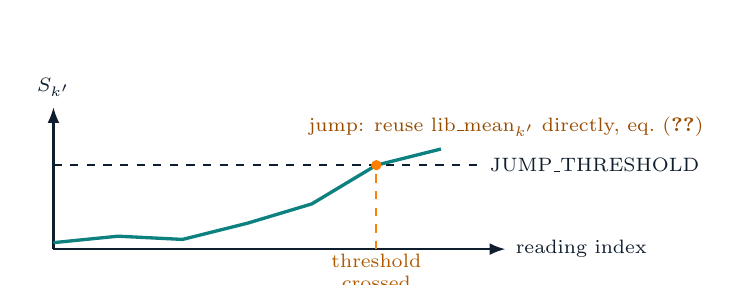
\begin{tikzpicture}[scale=0.82]
\draw[-{Latex[length=2mm]},thick,navy] (0,0) -- (7,0) node[right,font=\scriptsize]{reading index};
\draw[-{Latex[length=2mm]},thick,navy] (0,0) -- (0,2.2) node[above,font=\scriptsize]{$S_{k'}$};
\draw[navy,dashed,thick] (0,1.3) -- (6.6,1.3) node[right,font=\scriptsize]{JUMP\_THRESHOLD};
\draw[teal,very thick] plot coordinates {(0,0.1)(1,0.2)(2,0.15)(3,0.4)(4,0.7)(5,1.3)(6,1.55)};
\draw[orange,dashed,thick] (5,0) -- (5,1.3);
\filldraw[orange] (5,1.3) circle (2pt);
\node[orange!70!black,font=\scriptsize,align=center] at (5.0,-0.35) {threshold\\crossed};
\node[orange!60!black,font=\scriptsize,align=left,anchor=west] at (3.8,1.9) {jump: reuse $\text{lib\_mean}_{k'}$ directly, eq.~\eqref{eq:jump}};
\end{tikzpicture}
\end{center}
Before the crossing, $S_{k'}$ is free to wander back toward zero on contrary evidence
(the $\max(0,\cdot)$ floor and the per-step reset above) -- the flat, quiet stretch on
the left; only a sustained run earns the vertical snap on the right, and only then is
the library (Section~\ref{sec:library}) actually reused.

\subsection{The jump: discrete reuse}
\label{sec:jump}
When $S_{k'}$ exceeds \code{JUMP_THRESHOLD}, and only if $k'$'s library is mature
enough to trust ($\text{lib\_var}_{k'}<\text{LIB\_VAR\_INIT}$, i.e.\ it has been
confidently observed at least once before -- a jump is never made into an untouched,
default library entry):
\begin{equation}\label{eq:jump}
w_{k'}\leftarrow 0.85,\quad w_{k\ne k'}\leftarrow\frac{0.15}{K-1},\qquad
v_{k'}\leftarrow\text{lib\_mean}_{k'},\qquad
P_{k',vv}\leftarrow\max(\text{lib\_var}_{k'},\text{floor}),\qquad S\leftarrow0.
\end{equation}
This is the literal reuse step: the controller does not wait for enough further
evidence to let \eqref{eq:imm-mix} arrive at high confidence on its own; it resets
directly into the previously learned speed and a correspondingly tight (previously
earned) uncertainty, the moment accumulated evidence makes that trustworthy.

\subsection{Threshold selection on development data}
\label{sec:threshold-selection}
$(\text{slack},\text{JUMP\_THRESHOLD})$ were chosen by grid search on 50--100
development seeds of \code{repeated} (benefit) and \code{normal} (false-jump cost,
counted by direct instrumentation of calls to the jump routine, not an indirect proxy
such as a raw weight-delta threshold, which was tried first and found to conflate
ordinary noisy Bayesian swings with genuine jumps):
\begin{center}\small
\begin{tabular}{rrrr}\toprule
slack & threshold & reconvergence, visits 2+ (cm/s decisions) & false jumps / 100 \code{normal} trials\\\midrule
0.0 & 0.2 & $\approx2.1$ & 4\\
0.1 & 0.3 & $\approx2.2$--$2.4$ & 3\\
\textbf{0.2} & \textbf{0.5} & $\approx\mathbf{2.9}$--$\mathbf{3.1}$ & \textbf{1}\\
0.3 & 1.0 & $\approx4.5$ (little benefit) & 0\\
\bottomrule
\end{tabular}\end{center}
The chosen point (bold) trades a somewhat larger effect at $(0,0.2)$ for a
near-eliminated false-jump rate; it is a selected operating point, not the only one
examined, and the trade-off actually observed is reported here rather than only the
final choice.

\subsection{The result}
\label{sec:memory-result}
\begin{center}\small
\begin{tabular}{lrrr}\toprule
Visit & \code{ext1} & \code{ext1_memory} & \code{ext1_memory_fast}\\\midrule
1st (slow) & 4.3 (79/100) & 4.4 (77/100) & 4.4 (77/100)\\
2nd (slow) & 4.7 (80/100) & 4.9 (60/100) & \textbf{3.3 (87/100)}\\
3rd (slow) & 4.7 (68/100) & 4.9 (50/100) & \textbf{3.2 (83/100)}\\
\bottomrule
\end{tabular}\end{center}
The first visit is identical across all three, exactly as~\eqref{eq:jump}'s maturity
guard predicts: there is nothing to reuse yet. From the second visit onward,
\code{ext1_memory_fast} is both faster and more reliable (more trials converge at
all within the segment), with the gap widening on later visits. On \code{switch},
\code{recovery} and \code{normal} -- scenarios with no repeat visit within an episode --
all three policies are byte-identical in \code{results_ext1/summary.csv}: no cost, no
new false alarms, because there is nothing yet to recognise. This is a genuine,
reproducible confirmation of the governing hypothesis, reached only after the first
design (library alone) failed and was correctly diagnosed rather than abandoned or
silently re-tuned until it looked right.
\tutoext{7}{Context memory: a negative result, a diagnosis, and a fix}

\section{Breaking the distance/bias confound: an explicit reference}
\label{sec:bias-ref}
Section~\ref{sec:obs}'s observation model, $y_n=d_n+(b-\hat b)+\nu_n$, makes the point
precisely: from a single sensor's stationary readings alone, an unknown constant bias
$b-\hat b$ and an unknown true distance $d_n$ are not separately identifiable --
replacing $(d,b)$ by $(d+\delta,b-\delta)$ leaves every reading unchanged. No amount of
further filtering (Milestones 1-2) can resolve this; the \code{bias} scenario's fixed
$+5$~cm offset, never captured by the static calibration $\hat b$, is exactly this
failure mode, and it is the reason the information-seeking policies did noticeably
worse under it (Milestone 1's unresolved pattern).

\subsection{A known-distance reference, not a cleaner oracle}
\label{sec:bias-ref-method}
The only way to break the confound is a second, independent piece of information
about one of the two unknowns. \code{CognitiveController.calibrate_bias}, called once
before the main approach loop, takes $N_{\mathrm{ref}}=5$ readings of a fixed,
\emph{known} reference distance $d_{\mathrm{ref}}=50$~cm (chosen clear of the task's
own 25~cm target and 55--130~cm start range) through the \emph{same} noisy sensor
model used for the main task -- not a separate, cleaner channel, and never a read of
\code{simulator_true_distance}:
\begin{equation}\label{eq:ref-readings}
z_i=d_{\mathrm{ref}}+\beta+\nu_i,\qquad \nu_i\sim\N(0,R),\qquad i=1,\dots,N_{\mathrm{ref}},
\end{equation}
where $\beta$ is whatever deployment-time bias is actually present. Since $d_{\mathrm
{ref}}$ is known rather than estimated, any systematic offset in $\bar z=\tfrac1{N_
{\mathrm{ref}}}\sum_i z_i$ must be bias, not distance error -- this is precisely what
breaks the identifiability problem above. The estimator is an ordinary mean with its
standard error:
\begin{equation}\label{eq:bias-est}
\hat\beta=\bar z-\hat b-d_{\mathrm{ref}},\qquad \widehat{\mathrm{Var}}(\hat\beta)=R/N_{\mathrm{ref}}.
\end{equation}
At $R=1.44$~cm$^2$ and $N_{\mathrm{ref}}=5$, $\mathrm{se}(\hat\beta)\approx0.54$~cm --
small relative to the 5--8~cm biases tested below, so the reference should reliably
detect them, which the results confirm.

\subsection{Propagating the estimate and its uncertainty}
\label{sec:bias-ref-propagate}
\code{Belief.set_bias_reference}$(\hat\beta,\widehat{\mathrm{Var}}(\hat\beta))$
changes exactly two things in the belief, both defaulting to $(0,0)$ so every policy
without a reference is numerically unaffected: the bias correction in
\code{Belief.observe} becomes $y_n=z_n-\hat b-\hat\beta$, and every use of the
observation variance becomes $R\mathrel{+}=\widehat{\mathrm{Var}}(\hat\beta)$. This is
the "propagate its uncertainty into the stopping decision" requirement: the
reference's own imprecision inflates the effective sensor noise used by the existing
Kalman update everywhere it appears, which already correctly widens $P$ and therefore
the verification margin $|\mu-25|+1.64\sqrt P\leq4$ -- no change to the verification
rule itself was needed, only to what feeds it.

\subsection{Results}
\label{sec:bias-ref-result}
\code{ext1_bias_ref} (\code{ext1} plus the reference only -- not combined with
memory/fast-switch, to isolate this one factor) against plain \code{ext1}, on the
existing fixed-offset \code{bias} scenario and a new \code{bias_random} scenario
(a fresh $\mathrm{Uniform}(-8,8)$~cm draw per trial, testing whether the mechanism
generalises beyond the one offset \code{bias} happens to use):
\begin{center}\small
\begin{tabular}{lrrr}\toprule
Scenario & \code{ext1} success & \code{ext1_bias_ref} success & Mean $|\hat\beta-\beta|$\\\midrule
\code{bias} (fixed $+5$) & 86\% & \textbf{99\%} & 0.42 cm\\
\code{bias_random} ($\pm8$) & 53\% & \textbf{99\%} & 0.42 cm\\
\bottomrule
\end{tabular}\end{center}
\code{bias_random} is the more informative result: an uncorrected unknown bias is far
worse than the single fixed $+5$~cm case suggested (53\% vs.\ 86\% success), yet the
reference recovers to the same $\approx99\%$ regardless of the offset's size or sign,
for a cost of 5 decisions ($0.75$~s) charged separately from the main approach budget,
not against it. This also closes Milestone 1's open question: with the confound
actually broken, the information-seeking \code{ext1_bias_ref} is no longer at a
disadvantage under bias relative to a no-information comparator -- the earlier
vulnerability was about the confound, not about information-seeking as such.
\tutoext{8}{An explicit sensor-bias reference}

\section{Calibration}
\label{sec:calib}
Calibration is unchanged from the previous Extended-system release: sensor bias and variance from \code{calibration_sensor.csv} (seed 1701, four distances, the Baseline system's $\hat b,\hat R$ estimators in \code{baseline_v1/Mathematical_Model.pdf}, Section~11.1), and per-context speed $m_k=\overline{\ell_i/\tau_i}$ from \code{calibration_motion.csv}, pooled over 80 pulses per context. The single-sensor identifiability caveat is structural, not fixed by better filtering: $y=d+b+\nu$ does not separately identify $(d,b)$ from stationary data alone. Section~\ref{sec:bias-ref} adds an explicit, costed reference observation that resolves it when enabled; policies without that reference remain exactly as limited as described here.
\tutoVone{Section 11}{Calibration as parameter estimation}

\section{Default parameters: a complete reproducible specification}
\label{sec:defaults}
\small
\begin{longtable}{p{.40\linewidth}p{.18\linewidth}p{.32\linewidth}}
\toprule Configuration / quantity & Default & Interpretation\\\midrule\endhead
Duration menu $\{\tau\}$ & $\{0,.12,.24\}$~s & Shared by all cognitive policies and \code{FairRuleBaseline}\\
Planning horizon $H$ & 2 decisions & \code{CognitiveController._plan}\\
Cost weight & 0.08 & Per-step, both horizon steps\\
Information weight & 0.8 & First horizon step only\\
No-progress threshold $\Delta_{\min}$ & 1~cm & Net two-step displacement\\
No-progress penalty $\lambda$ & 1.0 & Added to the all-SAMPLE pair only\\
Overshoot margin & 2.33$\sigma$ + 0.5~cm & Both horizon steps, and \code{FairRuleBaseline}'s single step\\
Context transition $T$ & diag .96, off-diag .04 & \code{Belief._advance}; applied on motor decisions only\\
Speed mean-reversion $\rho$ & 0.80 (contexts), 1 (adaptive) & \code{Belief._advance}\\
Process variance $(Q_d,Q_v)$ & 0.04, 0.30 (contexts) / 0.65 (adaptive) & Added per motor decision\\
Innovation rejection & $5\sigma$ standardised & \code{Belief.observe}\\
Verification & $|\mu-25|+1.64\sigma\leq4$, 3 consecutive & Shared with the Baseline system's Mini policy\\
Budgets & 80~s, 100 moves, 350 decisions & Shared across all eight evaluated policies\\
Library confidence gate & $w_k>0.7$ & \code{Belief._update_library}, eq.~\eqref{eq:lib-update}\\
Library initial / floor variance & 4.0 / 0.05 & \code{LIB_VAR_INIT} / \code{LIB_VAR_FLOOR}\\
CUSUM slack / threshold & 0.2 / 0.5 & Selected on development data, Section~\ref{sec:threshold-selection}\\
Jump weight / variance floor & 0.85 / 0.05 & eq.~\eqref{eq:jump}\\
Reference distance / readings & 50 cm / 5 & \code{REF_DISTANCE} / \code{N_REF}, Section~\ref{sec:bias-ref}\\
\bottomrule
\end{longtable}
\normalsize
All values above were read from \code{cognitive/controller.py}, \code{cognitive/model.py}, \code{cognitive/baselines.py} and \code{tests/test_cognitive.py} at the time of writing, not retyped from an earlier draft.
\tutoVone{Section 13}{Default parameters: a complete reproducible specification}

\section{A frozen, held-out evaluation}
\label{sec:heldout}
Every result in Sections~\ref{sec:horizon}--\ref{sec:bias-ref} comes from seeds
10000--10099, and several of the constants in the table above (the CUSUM pair above
all) were explicitly selected by grid search \emph{on that same seed range}
(Section~\ref{sec:threshold-selection}). That is development-set reporting, not
independent confirmation. This section's entire job is evaluation, not architecture:
every constant above is frozen (recorded, with its file location, in \code{docs/
FROZEN_PARAMETERS.md}) and the full battery of policies and scenarios is re-run,
unmodified, on seeds 50000--50099 -- a range never used for development or tuning --
via \code{experiments/run_simulation.py --seed-start 50000 --out-dir
results_ext1_heldout}.

\subsection{An added robustness scenario: outliers}
\label{sec:outlier}
One gap was worth closing alongside the freeze: \code{dropout} tests \emph{missing}
readings, but nothing tested a reading that is \emph{present}, passes the basic
range check, yet is badly wrong -- the case the innovation-rejection gate
($\S$\ref{sec:obs}, $|{\rm innovation}|>5\sigma$) exists for. The new \code{outlier}
scenario corrupts each reading independently with probability $0.05$ by adding
$\mathrm{Uniform}(-20,20)$~cm, drawn from the same noise stream as the ordinary
sensor noise (the same physical sensor glitching, not a separate failure channel).
This is purely descriptive for this release: there was no prior claim about outlier
handling to confirm, only a new measurement.

\subsection{Replication report}
\label{sec:replication}
Comparing \code{results_ext1/} (development) against \code{results_ext1_heldout/}
(held-out), computed by \code{experiments/compare_heldout.py}:
\begin{center}\small
\begin{tabular}{lrr}\toprule
Claim & Development & Held-out\\\midrule
\code{v1_fair}/\code{v1} moves, \code{normal} (Milestone 1) & ratio 0.54 & ratio 0.54\\
No-information success/abort, \code{normal} (Milestone 1) & 100\% / 0\% & 100\% / 0\%\\
\code{ext1_memory_fast} reconv., visit 2 (Milestone 2) & 3.3 vs.\ 4.7 (\code{ext1}) & 3.2 vs.\ 4.6 (\code{ext1})\\
\code{ext1_bias_ref} success, \code{bias} (Milestone 3) & 86\%$\to$99\% & 78\%$\to$100\%\\
\code{ext1_bias_ref} success, \code{bias_random} (Milestone 3) & 53\%$\to$99\% & 52\%$\to$100\%\\
\bottomrule
\end{tabular}\end{center}
Every headline result replicates: the same ordering, and magnitudes close enough to
be ordinary sampling variation at $n=100$ (the \code{ext1} baseline under \code{bias}
moved from 86\% to 78\% between seed ranges -- noticeable, but the reference's
recovery is, if anything, slightly stronger on held-out seeds, so the qualitative
conclusion is unaffected). The new \code{outlier} scenario shows a mild, consistent
dip across most policies on held-out seeds (success $\approx$97--98\%$\to\approx$92--95\%,
aborts $\approx$2\%$\to$5--8\%) except \code{ext1_bias_ref}, which moved the other
direction -- within normal sampling noise for a 5\%-probability event at $n=100$, not
a systematic failure pattern tied to any one architecture.
\tutoext{9}{A frozen held-out evaluation}

\section{A cross-task transfer test: the Transfer system, and Objective O3}
\label{sec:transfer}
Every milestone above (Sections~\ref{sec:horizon}--\ref{sec:heldout}) is evaluated on
one task: approach a wall and verify 25~cm. This section tests a different question,
raised separately from the six-point improvement plan closed in
Section~\ref{sec:next}: does the per-context speed library built and validated in
Section~\ref{sec:cusum} -- a learned, reusable representation, recognised and
reapplied via the CUSUM mechanism -- transfer to a genuinely different goal, not just
to repeat visits of the same task? This is tested here as a self-contained,
additional validation pass, the \emph{Transfer system}, not as a seventh item of that
closed plan.

\subsection{Task B: the same physics, a different goal}
\label{sec:taskb}
Task A is unchanged: target $g_A=25$~cm, band $\beta=4$~cm, start
$\mathrm{Uniform}(55,80)$~cm ($\mathrm{Uniform}(100,130)$ for \code{repeated}).
\textbf{Task B}: target $g_B=85$~cm, band $\beta=4$~cm (same half-width), start
$\mathrm{Uniform}(115,145)$~cm -- clearly separated from both $g_A$ and the shared
bias-reference distance (50~cm, Section~\ref{sec:bias-ref}, unchanged). The
verification rule of Section~\ref{sec:verify} generalises directly to any target $g$:
\begin{equation}\label{eq:verify-general}
|\mu-g|+1.64\sigma\leq\beta,\quad\text{3 consecutive decisions for DONE.}
\end{equation}
Here, as in eq.~\eqref{eq:verify-v1}, $\mu,\sigma$ denote whatever the acting
controller's own belief reports as its distance mean and standard deviation --
$\bar d,\sqrt{\bar P_{dd}}$ (eq.~\eqref{eq:moments}) for \code{CognitiveController}'s
joint mixture, or the plain scalar belief for \code{FairRuleBaseline}, which tracks no
mixture at all (Section~\ref{sec:fair}). The verification \emph{form} is identical
either way; only which belief feeds it differs.
\code{CognitiveController} and \code{FairRuleBaseline} now take \code{target}/
\code{band} as constructor parameters (default 25/4, reproducing every earlier
result unchanged -- confirmed by re-running the full Section~\ref{sec:heldout}
battery and diffing every output byte-for-byte against its pre-change snapshot).
Task B deliberately reuses Task A's sensor and motor model unchanged -- same
normal/slow speeds, same per-trial noise -- so only the goal differs; transfer under
a genuinely different sensor or surface characteristic is left for a later pass.

\subsection{A persistent per-deployment speed bias}
\label{sec:checkpoint}
A first attempt at this test built one shared checkpoint (next paragraph's recipe,
without the bias introduced below) and reused it for all 100 Task-B seeds. It found
no measurable difference between any of the three conditions below. The reason,
traced directly rather than assumed: the checkpoint converged to
$(\text{lib\_mean}_{\text{normal}},\text{lib\_mean}_{\text{slow}})=(7.81,3.34)$~cm/s,
within noise of the untrained calibration prior $(8.0,3.0)$ that a cold-start belief
already uses as eq.~\eqref{eq:advance}'s reversion target. Task A's \code{repeated}
scenario draws its true speeds from exactly those same calibration constants (only a
per-trial $\mathrm{Uniform}(0.9,1.1)$ factor, which averages out), so a library
trained on it mostly rediscovers what calibration already supplied for free -- there
was no information gap left for cross-task transfer to close. The seeding mechanism
itself was independently confirmed working by unit test (a frozen, seeded library is
correctly read by \code{_advance} and \code{_jump_to}); the task design, not the
mechanism, is what gave it nothing to do.

This version fixes that by giving Task A something to teach that calibration cannot
already supply: each of the 100 standard seeds is now its own \emph{deployment}, with
a persistent multiplicative speed bias
$\gamma\sim\mathrm{Uniform}(0.6,0.85)$ (frozen in \code{docs/FROZEN_PARAMETERS.md},
drawn deterministically from the seed before any run, not after seeing results) --
clearly outside both the existing per-trial factor's range and the calibration
estimator's own sampling noise (the pooled 80-pulse mean's standard error is
$\approx$0.056~cm/s, two orders of magnitude tighter). $\gamma$ multiplies true speed
in \emph{both} that deployment's Task A training and its Task B evaluation, composed
into the existing per-trial factor at \code{episode()}'s one call site
($\text{factor}=\mathrm{Uniform}(0.9,1.1)\times\gamma$, default $\gamma=1$ an exact
no-op, confirmed by re-running the full held-out battery byte-for-byte unchanged) --
but is invisible to \code{calibrate()}'s static estimate, which only ever sees the
80-pulse calibration population, never a deployment's $\gamma$. A cold-start belief on
Task B therefore now starts from a provably wrong prior; a checkpoint trained on that
same deployment's Task A should already know the correction.

For each deployment, \code{ext1_memory_fast} (Section~\ref{sec:cusum}) is run on Task
A's \code{repeated} scenario, under that deployment's own $\gamma$, across successive
independent episodes (position filter and CUSUM accumulator reset between them, as
before; only $(\text{lib\_mean}_k,\text{lib\_var}_k)$ persists), until both contexts'
library entries are mature ($\text{lib\_var}_k<\text{LIB\_VAR\_INIT}$, eq.~\eqref{eq:jump}'s
own gate). All 100 deployments matured within a single 100-move \code{repeated}
episode, as in the first pass.

\subsection{Three conditions on Task B}
\label{sec:conditions}
Each of the 100 deployments is evaluated on both Task B scenarios (\code{normal}:
constant context; \code{switch}: also exercises the slow-context entry and the
fast-recognition mechanism, Section~\ref{sec:cusum}), under its own $\gamma$ in every
condition -- cold-start faces the identical real bias, it simply never learned it
from Task A first:
\begin{itemize}
\item \textbf{Cold start.} A fresh \code{ext1_memory_fast} controller, empty
library -- the comparison baseline.
\item \textbf{Zero-update transfer.} Library seeded from that deployment's checkpoint;
the \code{memory_frozen} flag on \code{Belief} gates eq.~\eqref{eq:lib-update}'s call
site ($\text{if memory and not memory\_frozen}$), so the seeded values are still read
by eq.~\eqref{eq:advance} and eq.~\eqref{eq:jump} but never rewritten -- transfer
without adaptation, exactly as O3 separates the two.
\item \textbf{Adaptation with updates.} Same seeded starting point,
\code{memory_frozen=False} -- transfer, with adaptation left on.
\end{itemize}
\code{memory_frozen} defaults to \code{False} and is inert unless a library is both
present and explicitly frozen, so every earlier policy and result is numerically
unaffected -- confirmed by the existing test suite plus new tests (non-regression of
the \code{target}/\code{band} defaults and of $\gamma=1$'s default; a non-default
target/band shifting the verification boundary; $\gamma$ correctly scaling the
simulated true speed; a direct unit test seeding $\text{lib\_mean}$/$\text{lib\_var}$
into a frozen belief and confirming it is read without being rewritten).

\subsection{Results: still nothing on the original metrics}
\label{sec:transfer-result}
Decisions-to-target: the first decision at which eq.~\eqref{eq:verify-general} holds
(a single crossing, not the 3-consecutive DONE criterion).
\begin{center}\small
\begin{tabular}{llrrrr}\toprule
Condition & Scenario & Success & Mean moves & Reached band & Decisions-to-target\\\midrule
Cold start & \code{normal} & 100\% & 27.5 & 100\% & 28.89\\
Zero-update transfer & \code{normal} & 100\% & 27.4 & 100\% & 28.89\\
Adapt with updates & \code{normal} & 100\% & 27.5 & 100\% & 28.90\\\addlinespace
Cold start & \code{switch} & 98\% & 46.1 & 100\% & 47.83\\
Zero-update transfer & \code{switch} & 97\% & 46.0 & 100\% & 47.77\\
Adapt with updates & \code{switch} & 97\% & 46.1 & 100\% & 47.90\\
\bottomrule
\end{tabular}\end{center}
Despite a real, substantial persistent bias ($\gamma\in[0.6,0.85]$, confirmed by a
traced example to leave cold-start and zero-update-transfer's belief trajectories and
action sequences essentially identical from the first decision onward), these four
metrics still show no measurable difference. The reason, again traced rather than
assumed: the sensor is precise (1.2~cm noise) relative to the distances involved, so
the Kalman update of Section~\ref{sec:update} locks onto the true (biased) speed from
direct position readings within one or two decisions, regardless of whether
eq.~\eqref{eq:advance}'s reversion target started at the correct, transferred value or
the generic calibration default -- the reversion pull ($\rho=0.8$, 20\%/step) is too
weak next to that fast evidence-driven correction to change any discrete planner
decision. Decisions-to-target then measures mostly the 30--60~cm of remaining travel,
which swamps any one- or two-decision transient at this scale.

\subsection{A sharper metric: post-switch reconvergence}
\label{sec:switch-reconvergence}
Section~\ref{sec:diagnosis} already identified the one place this architecture's
library demonstrably helps: not estimation precision of a directly, continuously
observed scalar, but \emph{recognition} delay when a regime must be distinguished
from a competing one -- exactly Section~\ref{sec:memory-result}'s reconvergence
result. Decisions-to-target cannot see this because it is a distance-to-goal metric;
isolating recognition requires the same definition \code{reconvergence_times} already
uses in Section~\ref{sec:memory-result} (tol $=1.5$, sustain $=3$), applied here to
Task~B's \code{switch} scenario's one regime change (\code{moves_completed}$\,\geq 12$):
decisions from the switch until the estimated speed is within tolerance of the new
true speed for 3 consecutive decisions.
\begin{center}\small
\begin{tabular}{lr}\toprule
Condition & Mean decisions to reconverge, post-switch\\\midrule
Cold start & 5.20\\
Zero-update transfer & \textbf{3.79}\\
Adapt with updates & \textbf{3.85}\\
\bottomrule
\end{tabular}\end{center}
This is a real, consistent effect, not an artefact of the mean: paired by deployment
($n=100$, every deployment contributing one cold-start and one zero-update-transfer
value), zero-update transfer reconverges faster in 61 deployments, ties in 32, and is
slower in only 7, for a mean paired reduction of 1.41 decisions
($\mathrm{se}=0.19$, $t\approx7.5$). The magnitude and direction match
Section~\ref{sec:memory-result}'s own within-task result (4.7$\to$3.3 decisions on a
second visit) closely enough to be the same mechanism, now shown surviving a change of
goal and a persistent, calibration-invisible speed bias -- not merely a repeated
observation of the same context within one episode. Adapt-with-updates (3.85) does no
worse than zero-update transfer (3.79): adaptation is not costing anything when the
transferred prior already happens to be useful, the second half of O3's own
"transfer without updates / adaptation with updates" distinction.

\subsection{Conclusion: positive preliminary evidence for O3, with its actual scope}
\label{sec:transfer-diagnosis}
Taken together, this \textbf{is} positive preliminary evidence for Objective O3, but
for a narrower claim than "transfer helps the robot finish the task faster": the
context library transfers across a genuine change of goal and deployment, and it
measurably speeds up the one thing it was ever shown to speed up --
recognising which movement regime is currently active -- while leaving overall
task completion statistically unchanged, because this architecture's direct,
low-noise position filtering already recovers a correct speed estimate within a
couple of decisions regardless of the starting prior. Both halves are reported
together deliberately: claiming only the positive metric would overstate what
transferred; claiming only the null metrics (as the first pass, honestly, had to)
would have missed where the effect actually lives.
\tutoext{11}{The Transfer system: a cross-task test of O3}

\section{Reading route and tutorial crosswalk}
\begin{longtable}{p{.34\linewidth}p{.20\linewidth}p{.34\linewidth}}
\toprule Mathematical question & This companion & Extended-system tutorial section\\\midrule\endhead
What changed and why? & Sections 1, 6--8 & 1, 7, 8\\
How is the joint belief defined and propagated? & Sections 2, 4 & 3\\
How does a reading update distance, speed and context? & Section 5 & 3\\
What is the information proxy? & Section 6 & 3--4\\
Why did the old planner risk stalling, and what replaces it? & Sections 7--8 & 4\\
How is the Baseline system given a fair comparison? & Section 9 & 4, 6--7\\
Why doesn't a persistent library alone speed up reuse? & Sections~\ref{sec:memory-negative}--\ref{sec:diagnosis} & 7\\
How does accumulated-evidence recognition fix it? & Section~\ref{sec:cusum} & 7\\
How is the distance/bias confound broken? & Section~\ref{sec:bias-ref} & 8\\
Do the results hold on data never used in development? & Section~\ref{sec:heldout} & 9\\
Does the learned context library transfer to a different goal (O3)? & Section~\ref{sec:transfer} & 11\\
Where do the numbers come from? & Sections~\ref{sec:calib}--\ref{sec:defaults} (Calibration; Default parameters) & 5\\
How do I reproduce the worked examples? & Sections~\ref{sec:worked-horizon}, \ref{sec:diagnosis} & 5--7\\
\bottomrule
\end{longtable}
\textbf{Practical links:} \href{Tutorial_EXT1_EN.pdf}{Extended-system PDF tutorial}; \href{README.md}{Extended-system README}; \href{baseline_v1/Mathematical_Model.pdf}{the Baseline system's mathematical companion} for the shared sensor and motor-mapping derivations; \href{Mini_IPHOREOS_EXT1_Video/EXT1_Explanation_EN.mp4}{Milestone~1}, \href{Mini_IPHOREOS_EXT1_Video/EXT1_Memory_Explanation_EN.mp4}{Milestone~2} and \href{Mini_IPHOREOS_EXT1_Video/EXT1_BiasHeldout_Explanation_EN.mp4}{Milestones~3--4} videos for captioned walkthroughs.

\textbf{Implementation authority:} \code{cognitive/model.py} (\code{Belief}), \code{cognitive/controller.py} (\code{CognitiveController}, including \code{_plan}), \code{cognitive/baselines.py} (\code{FairRuleBaseline}), and \code{experiments/run_simulation.py} for the evaluation protocol. This document describes the current implementation; it does not propose a different one.

\textbf{Rebuild/check:} from the \code{Mini_IPHOREOS_EXT1} directory, run the following command twice to resolve cross-references.
{\small
\begin{verbatim}
pdflatex -interaction=nonstopmode -halt-on-error Mathematical_Model_EXT1.tex
\end{verbatim}
}

\section{Status: all six improvement-plan items addressed}
\label{sec:next}
This release closes the project's own six-point improvement plan: fair comparators
(Section~\ref{sec:fair}), a short-horizon planner (Section~\ref{sec:horizon}), a
reusable per-context memory (Section~\ref{sec:library}), evidence-based change
detection (Section~\ref{sec:cusum}), an explicit sensor-bias reference
(Section~\ref{sec:bias-ref}), and a frozen held-out evaluation
(Section~\ref{sec:heldout}). Two of the six (memory and change detection) were
reached only after a first attempt was correctly diagnosed as insufficient and
redesigned, not on the first try, and the held-out evaluation exists specifically
because the other five were developed and tuned on a single, reused seed range --
closing the plan is not the same claim as closing every caveat raised along the way.

What this status explicitly does not mean: no physical robot has been built,
calibrated or tested: every result above is a desktop simulation. The verification
rule's three-consecutive-pass criterion remains correlated, not three independent
checks; paired bootstrap intervals remain descriptive and unadjusted for
multiplicity; the outlier and bias-random scenarios are new, single-release
measurements, not independently replicated beyond the one held-out seed range
reported here. \href{Tutorial_EXT1_EN.pdf}{The Extended-system tutorial}, Section~10, sets out
concretely what moving from this simulation to a physical trial would require.

Separately, Section~\ref{sec:transfer}'s Transfer-system pass found positive
preliminary evidence for Objective O3: under a persistent, calibration-invisible
per-deployment speed bias, a library trained on Task A measurably speeds up regime
recognition on Task B (post-switch reconvergence 5.2$\to$3.8 decisions, paired over
100 deployments), while overall success/moves/decisions-to-target stay unchanged --
reported as both halves together, not the favourable one alone.

\end{document}
